% ============================================================
% I. GIỚI THIỆU
% ============================================================
\section{Giới thiệu}

\begin{frame}{Bối cảnh: Học máy trong ngành thực phẩm}
      \begin{itemize}
        \item Các công đoạn trong công nghiệp thực phẩm đang chuyển từ xử lý thủ công sang hệ thống dựa trên dữ liệu ảnh \cite{mahalik2010trends,stemmer2018vision}.
        \item Công nghệ học máy có thể hỗ trợ theo dõi dinh dưỡng, bếp thông minh, kiểm soát chất lượng và tự động hóa vận hành \cite{gao2019smartfridge,wang2019smartrefrigerator}.
        \item Để dùng được trong thực tế, mô hình cần vừa \textbf{đủ chính xác} vừa \textbf{đủ nhẹ} cho suy luận nhanh.
      \end{itemize}

      \begin{block}{Thách thức đặc thù ảnh thực phẩm}
        Ranh giới mờ, texture gần nhau và thành phần chồng lấp khiến bài toán phân đoạn fine-grained khó hơn nhiều benchmark phổ biến.
      \end{block}
    
\end{frame}

\begin{frame}{Bài toán: nguyên lí, input và output}
      \textbf{Phát biểu bài toán:} dự đoán lớp cho \emph{từng pixel}, sau đó ghép lại thành bản đồ phân đoạn hoàn chỉnh.\\
      \vspace{0.25em}
\textbf{Input}: ảnh RGB $\mathbf{X}\in\mathbb{R}^{H\times W\times 3}$.\\
\textbf{Output}: mặt nạ nhãn pixel-level $\mathbf{Y}\in\{1,\dots,K\}^{H\times W}$.
      \vspace{0.25em}
      \begin{columns}[T,onlytextwidth]
        \column{0.40\textwidth}
        \textbf{Biểu diễn toán học}
        \[
          f_\theta:\mathbf{X}\to\mathbf{Y}
        \]
        \[
          \mathbf{Y}(i,j)=\arg\max_c\,p_\theta(c\mid\mathbf{X},i,j)
        \]

        \column{0.49\textwidth}
        \vspace{2em}
             $(i,j)$: chỉ số pixel theo hàng và cột.\\
             $c$: chỉ số lớp trong tập $\{1,\dots,K\}$.\\
            $p_\theta(c\mid\mathbf{X},i,j)$: xác suất pixel $(i,j)$ thuộc lớp $c$.
\      \end{columns}

      \vspace{0.35em}
      \begin{block}{Mục tiêu mô hình}
        Tối ưu đồng thời nhận diện đúng \textbf{lớp} và định vị đúng \textbf{biên/vùng} của nguyên liệu. Đáng chú ý, các vùng nhỏ và vùng biên thường là nơi mô hình lightweight suy giảm mạnh nhất.
      \end{block}
\end{frame}

\begin{frame}{Giới thiệu dataset: FoodSeg103}
  \begin{columns}
    \column{0.55\textwidth}
      \begin{block}{Thông tin chính}
        \begin{itemize}
          \item 7.118 ảnh thực phẩm, 103 lớp gốc \cite{benchmarkfood}
          \item 42.097 vùng mask được gán nhãn \cite{benchmarkfood}
          \item Bài toán fine-grained với nhiều lớp có texture tương tự
        \end{itemize}
      \end{block}

      \begin{alertblock}{Ý nghĩa với đề tài}
        Tập dữ liệu đủ khó để đánh giá rõ giới hạn của baseline lightweight bởi sự phức tạp về \textbf{texture}, \textbf{biên} và \textbf{mất cân bằng lớp} của tập dữ liệu.
      \end{alertblock}
    \column{0.4\textwidth}
      \begin{figure}
        \centering
        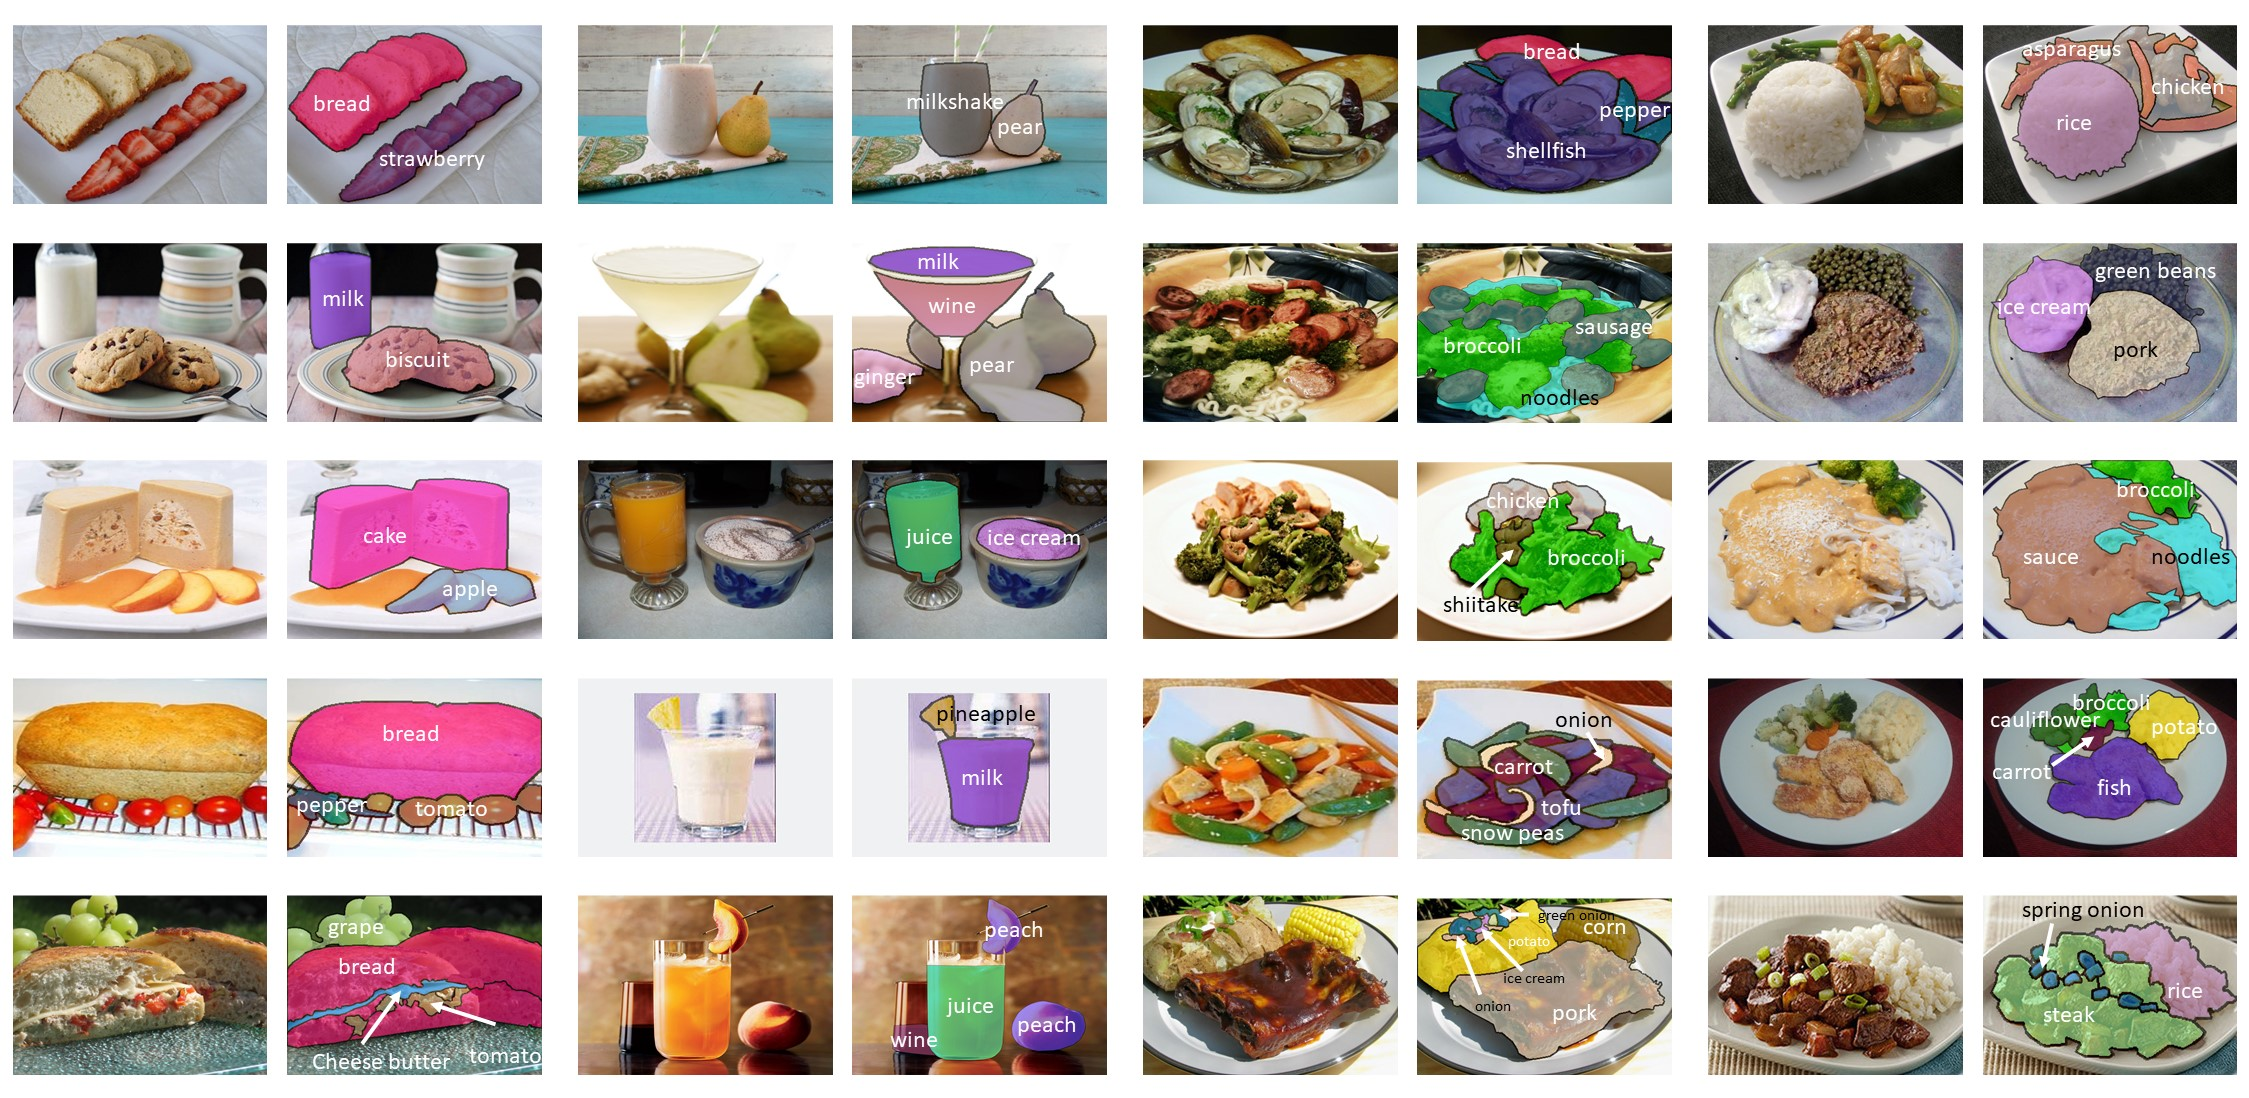
\includegraphics[width=\linewidth]{img/report/foodseg103.png}
        \caption{Mẫu ảnh trong FoodSeg103}
      \end{figure}
  \end{columns}
\end{frame}

\begin{frame}{Hàm mất mát và Chỉ số đánh giá}
%   \begin{columns}
%     \column{0.5\textwidth}
      \textbf{Pixel-wise Cross-Entropy}
      \[
        \mathcal{L}_\text{CE} = -\frac{1}{|\Omega|}\sum_{(i,j)\in\Omega}\log p_{i,j,y_{i,j}}
      \]
    % \column{0.48\textwidth}
      \textbf{Ba chỉ số đánh giá}
      \begin{align*}
        \text{mIoU} &= \tfrac{1}{K}\sum_c\tfrac{TP_c}{TP_c+FP_c+FN_c}\\
        \text{mAcc} &= \tfrac{1}{K}\sum_c\tfrac{TP_c}{TP_c+FN_c}\\
        \text{aAcc} &= \tfrac{\sum_c TP_c}{\sum_c(TP_c+FN_c)}
      \end{align*}
      \small mIoU là chỉ số chính vì nhạy với mất cân bằng lớp
%   \end{columns}
\end{frame}

\begin{frame}{Đóng góp và phạm vi thực nghiệm}
    \textbf{Ba đóng góp chính}
      \begin{enumerate}
        \item \textbf{Phân tích định lượng} bộ FoodSeg103: độ khó theo lớp, theo ảnh và theo cấu trúc lỗi.
        \item \textbf{Chuẩn hóa baseline BiSeNet} trực tiếp trên \textbf{FoodSeg103 nguyên thủy (103 lớp)} làm mốc tham chiếu cho các cải tiến tiếp theo.
        \item \textbf{Thiết kế nhánh thực nghiệm mở rộng} để kiểm tra tác động của tái cấu trúc nhãn (ngoài phạm vi baseline chính).
      \end{enumerate}
\vspace{0.25em}
%   \begin{columns}
%     \column{0.46\textwidth}
      \begin{alertblock}{Phạm vi báo cáo}
            Chọn một baseline lightweight, thực hiện phân tích lỗi chi tiết để hiểu rõ hơn về các hạn chế của mô hình, và đề xuất phương pháp khắc phục để tăng hiệu suất.

      \end{alertblock}
    % \column{0.46\textwidth}
    %   \begin{block}{Đầu ra mong muốn}
    %     \begin{itemize}
    %       \item baseline minh bạch
    %       \item chỉ số tin cậy
    %       \item hướng cải tiến cụ thể
    %     \end{itemize}
    %   \end{block}
%   \end{columns}
\end{frame}
